\section{Spieler-Interface}

% Aus dem Wiki
% ------------
%
% Siehe: https://sopra.informatik.uni-freiburg.de/soprawiki/index.php?title=GDD#Spieler-Interface
%
% Dieser Abschnitt beinhaltet eine Beschreibung des Spielbildschirms, also
% dessen, was für den Spieler sichtbar ist. Dies beinhaltet die Art der
% Darstellung (2D oder 3D), die Kamerasicht, usw.
%
% Wichtig ist, dass alle sichtbaren Elemente, wie Minimap, Menüleiste, etc.
% erklärt werden. Durch ein Bild eines typischen Vertreters dieser Spielart
% oder durch eine Konzeptzeichnung des Interfaces kann die Beschreibung noch
% verbessert werden. In der finalen Version des GDDs können auch Screenshots
% des eigenen Spiels verwendet werden.
%
% Außerdem wird in diesem Abschnitt erklärt, wie der Spieler das Spiel steuert
% (mit der Maus, mit Maus und Tastatur, Joystick, Gamepad usw.). Alle Aktionen,
% die der Spieler durchführen kann, müssen erklärt werden. Auch mögliche
% Shortcuts und/oder Tastenkombinationen sollten hier erwähnt werden.
%
%
% Aus den Folien
% --------------
%
% Siehe: https://sopra.informatik.uni-freiburg.de/soprawiki/images/1/11/How-To-GDD_SS19.pdf
%
% * Beschreibung dessen, was der Spieler sieht
% * Art der Darstellung, Kameraansichten, sichtbare Elemente (HUD, Minimap,
%   Menüleisten, usw.)
% * Bild (Konzeptzeichnung, Screenshot, Mockup) dessen, wie das Spiel aussehen
%   soll.
% * Beschreibung der Steuerung.

\missingSection{spieler-interface}

\begin{figure}[ht]
	\centering
	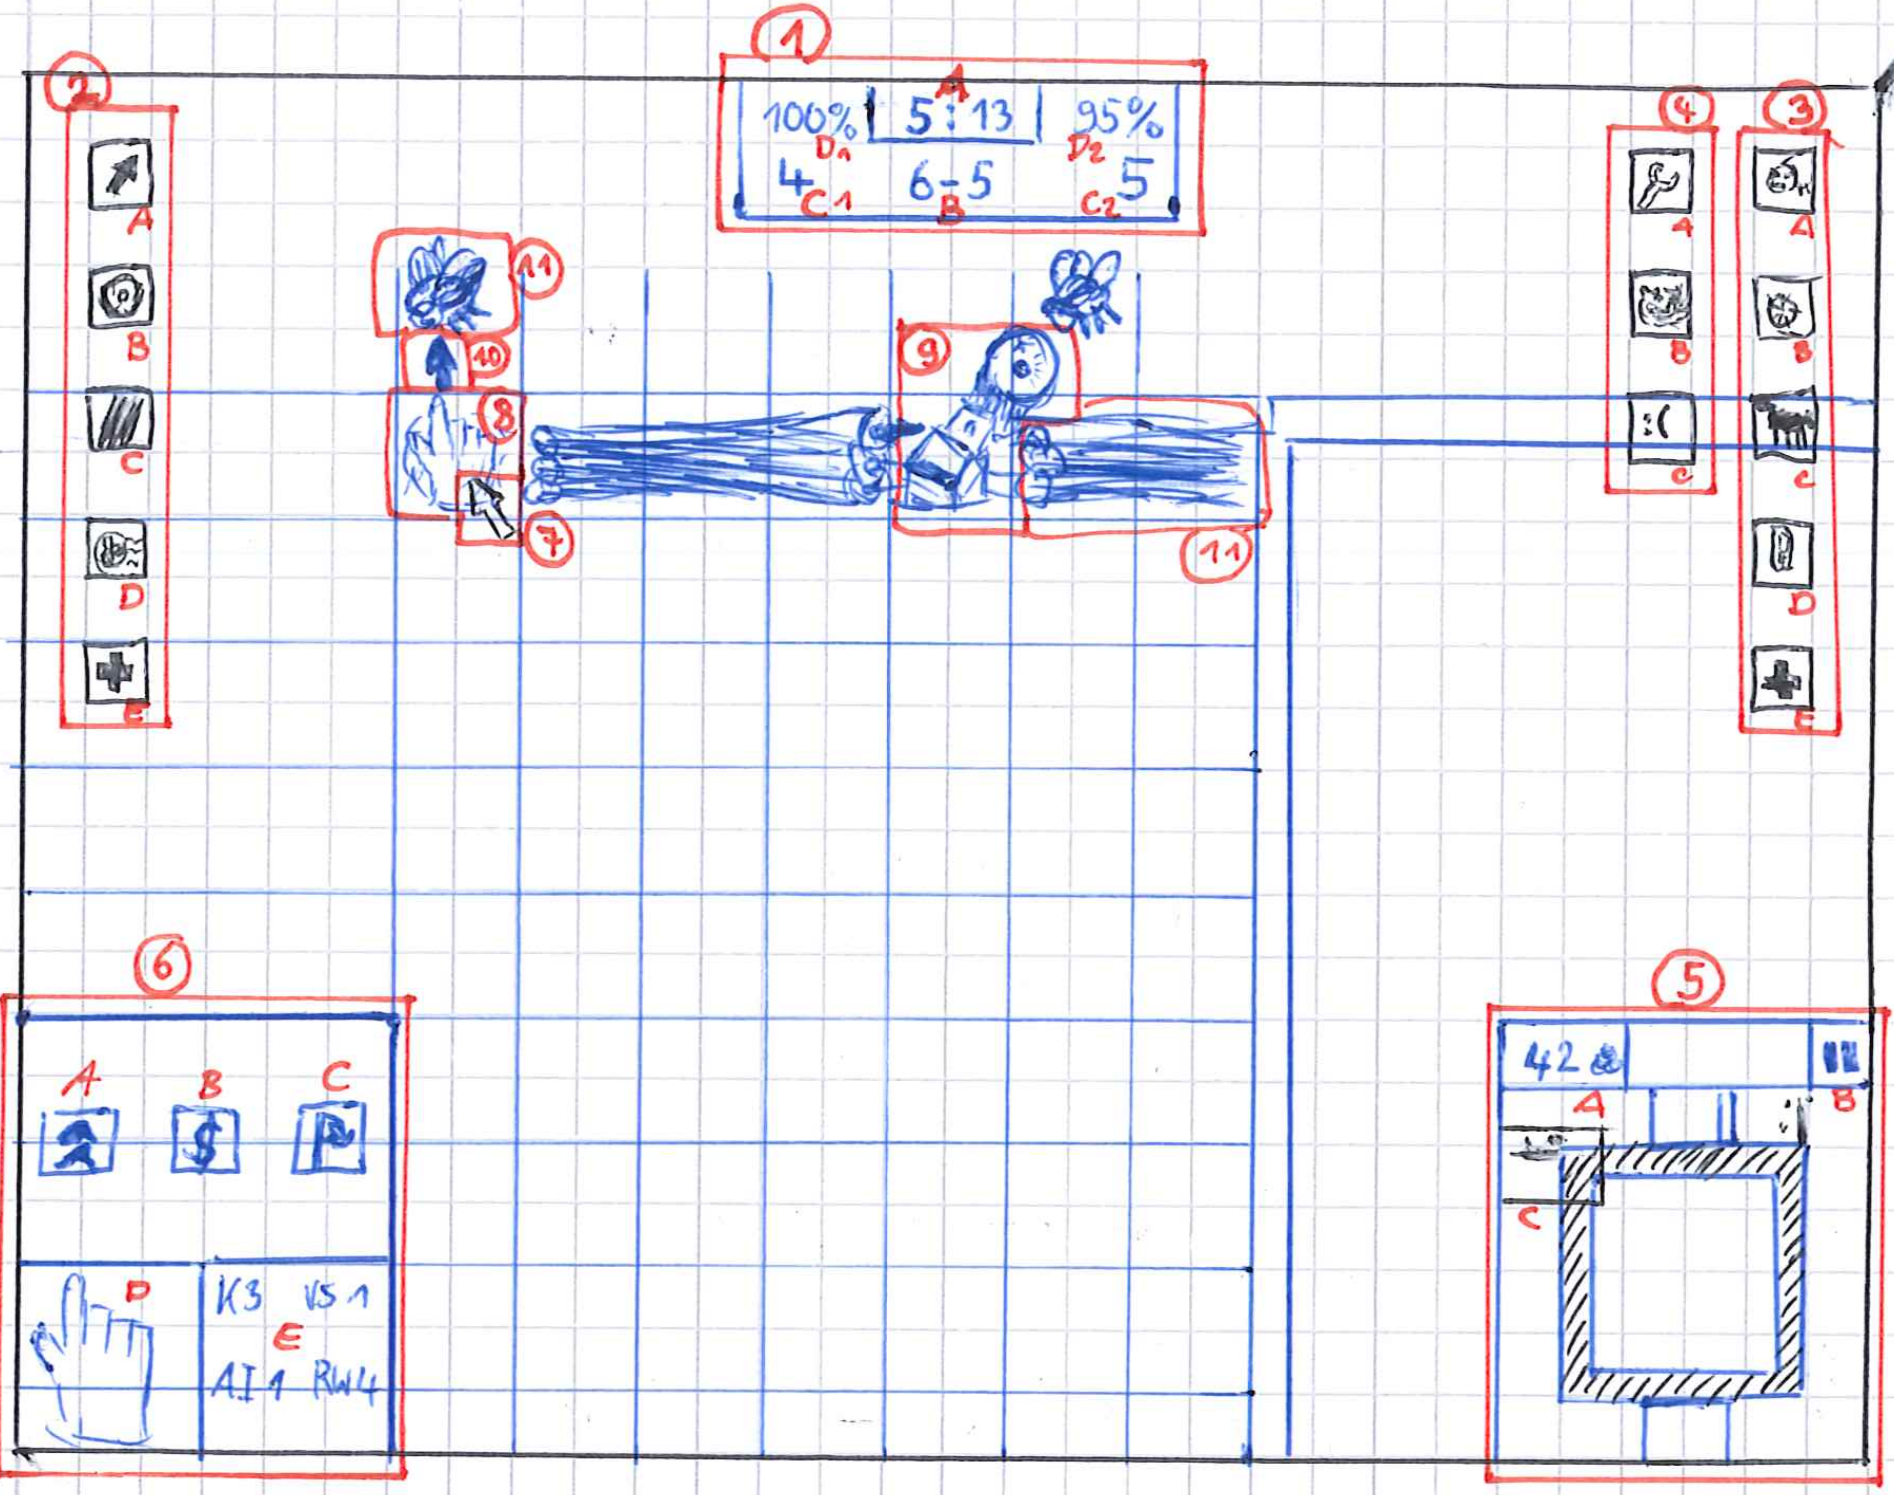
\includegraphics[width=1\textwidth]{spieler-interface.png}
	\caption{Spieler-Interface}
	\label{fig:spieler-interface}
\end{figure}
